% ID: SEL-D0011-BB-E04
% ESTADO: validada. S012; tres pasadas del mismo autor, sin segundo revisor.
\textbf{a.1) Gráfica de la derivada.}\par\nopagebreak[4]
La parábola con raíces $-4$ y $4$ tiene ecuación $f'(x)=k(x+4)(x-4)$. Su valor en $0$ es $8$, luego $-16k=8$ y $k=-1/2$:
\[
\boxed{f'(x)=8-\frac{x^2}{2}.}
\]
Abre hacia abajo, con vértice $(0,8)$ y las dos raíces indicadas. La curva representada es $f'$, no $f$.
\begin{center}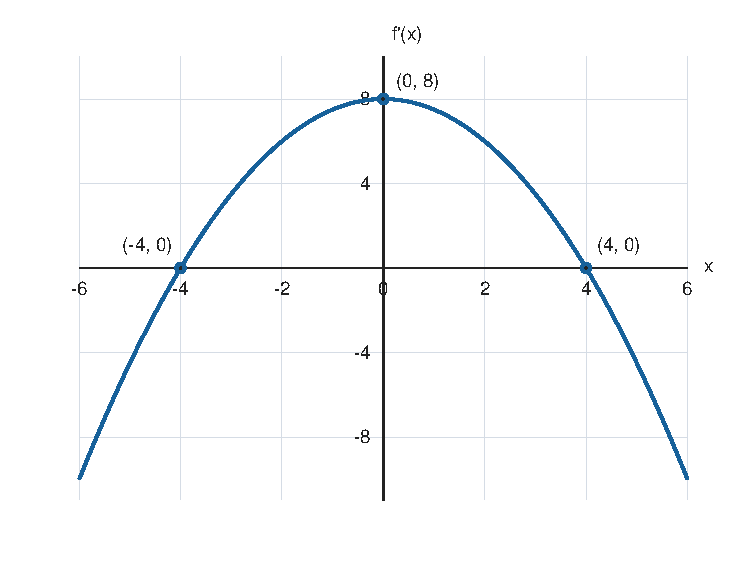
\includegraphics[width=0.57\linewidth]{recursos/figuras/s012-derivada.pdf}\end{center}

\textbf{a.2) Monotonía y extremos relativos de f.}\par\nopagebreak[4]
El signo de $f'$ es negativo fuera de $[-4,4]$ y positivo entre las dos raíces. Por tanto, $f$ decrece en $(-\infty,-4)$ y $(4,+\infty)$, y crece en $(-4,4)$.
En $x=-4$ la derivada pasa de negativa a positiva: \textbf{mínimo relativo}. En $x=4$ pasa de positiva a negativa: \textbf{máximo relativo}. Se piden sus abscisas; no se confunden las raíces de $f'$ con ceros de $f$.

\textbf{a.3) Tangente en el origen.}\par\nopagebreak[4]
El dato de paso por el origen da $f(0)=0$, y la pendiente es $f'(0)=8$. La ecuación punto-pendiente es
\[
y-f(0)=f'(0)(x-0)\quad\Longrightarrow\quad\boxed{y=8x.}
\]
Para comprobar la coherencia, una primitiva de $f'$ que pasa por el origen es $f(x)=8x-x^3/6$; su derivada y su tangente reproducen los datos.

\textbf{b) Derivada del producto.}\par\nopagebreak[4]
Se usa la regla del producto y la cadena en la exponencial:
\[
\begin{aligned}
g'(x)&=2x\,e^{2x-1}+(x^2-3)\,2e^{2x-1}\\
&=\boxed{2(x^2+x-3)e^{2x-1}.}
\end{aligned}
\]
Está definida para todo $x\in\mathbb R$.
